\documentclass[journal]{IEEEtran}
\usepackage{amsmath,amssymb,booktabs,array,multirow,url,cite,balance,graphicx}
\usepackage[hidelinks]{hyperref}

\title{An Empirical Study of Neural Representations and Benign-Only Anomaly Detection for Unknown Attacks in In-Vehicle CAN Traffic}
\author{Adda~Surendra, Gera~Vignan, and Vundadi~Mani~Kumar%
\thanks{The authors are with the Department of Computer Science and Engineering (Data Science and Artificial Intelligence), Indian Institute of Information Technology Design and Manufacturing, Kancheepuram, India (e-mail: surendraadda@gmail.com; gvignankv@gmail.com; vundadimanikumar@gmail.com). This project was carried out under the guidance of Dr. Bhale Pradeepkumar Gajendra, Assistant Professor, Department of Computer Science and Engineering, IIITDM Kancheepuram.}}
\markboth{Research Project Manuscript, November 2026}{Surendra \MakeLowercase{\textit{et al.}}: Neural Representations for Unknown CAN Attacks}

\begin{document}
\maketitle

\begin{abstract}
An in-vehicle intrusion detector is often trained with a finite set of attack labels, whereas a deployed vehicle may encounter traffic patterns that were not represented during training. This study examines one practical response to that mismatch: train a multilayer perceptron (MLP) to classify known Controller Area Network (CAN) traffic classes, use its 64-dimensional hidden activations as a representation, and fit an Isolation Forest (IF) to benign training representations. The experiments use the public CAN-train-and-test v1.5 data and treat six attack families in an evaluation capture as unknown to the six-class MLP. At the primary operating point, defined by the 99th percentile of benign calibration scores, the detector obtains 30.68\% precision, 19.00\% recall, and a 23.47\% F1-score, with a 1.04\% false-positive rate. Its continuous scores yield ROC-AUC 0.9423 and PR-AUC 0.4299. The family-wise results are uneven: 65.27\% of FUZZING records are detected, while no DOUBLE, INTERVAL, SPEED, or TRIPLE records cross the primary threshold. A 97.5th-percentile operating point produces 49.37\% F1 and 62.53\% recall, but it is retained as exploratory because the same unknown-test file had been examined during earlier threshold analysis. The comparison with an Isolation Forest fitted to the original features shows a distinction between ranking and thresholded decisions: the learned representation improves ROC-AUC and PR-AUC, but not F1 at the primary threshold. These results do not establish a new general-purpose detector or a complete reproduction of FedGAN-ID. They provide a reproducible account of one MLP--IF pipeline, its operating-point sensitivity, and the attack families it fails to identify.
\end{abstract}

\begin{IEEEkeywords}
Automotive cybersecurity, Controller Area Network, in-vehicle network, intrusion detection, unknown attacks, anomaly detection, neural representation, Isolation Forest.
\end{IEEEkeywords}

\section{Introduction}
A modern passenger vehicle is not a single computer. It is a collection of electronic control units (ECUs) that exchange short messages to coordinate functions such as engine management, braking, steering, body electronics, and driver assistance. The Controller Area Network (CAN) is one of the communication technologies used for this exchange. Its design favours timely, compact broadcast communication rather than the security properties normally associated with networks exposed to untrusted participants. In particular, a classical CAN frame does not by itself authenticate the ECU that transmitted it. An attacker who gains a route onto the in-vehicle bus may therefore attempt to inject frames, replay observed messages, or impersonate the traffic of another component. The security implications of such access have been demonstrated in automotive security research and motivate monitoring at the network level \cite{bosch1991can,rajapaksha2023survey,cho2016fingerprinting}.

An intrusion detection system (IDS) can complement preventive controls by observing bus activity and reporting behaviour that departs from an expected profile. CAN IDS research has considered several kinds of evidence. Some methods examine message identifiers and payload bytes; others model frame frequency, inter-arrival time, message ordering, or ECU-specific timing characteristics. These signals are related, but they are not interchangeable. A denial-of-service attack may create a pronounced rate change, whereas a masquerade or replay-like pattern may preserve a familiar identifier or approximate a legitimate transmission schedule. Timing-based methods can be useful when normal periodicity is stable, while content-oriented approaches can detect payload changes that a rate-only monitor would not see \cite{muter2011entropy,cho2016fingerprinting,rajapaksha2023survey}.

A common experimental assumption is that the attack classes available during training are also the classes that matter at evaluation time. That assumption is convenient for closed-set classification, but it does not describe the full operational problem. Attack variants change, and a vehicle manufacturer may not possess labelled examples of every malicious behaviour before deployment. An IDS intended to recognise previously unseen attacks must therefore do more than assign a test message to one of the labels learned during training. It needs a mechanism for identifying observations that are sufficiently unlike the benign operating region, while keeping false alarms at a usable level.

This paper studies a small, testable pipeline for that setting. A supervised MLP is trained on six known classes. The penultimate hidden activation is then treated as a compact representation of each CAN record. An Isolation Forest is fitted only to the hidden representations of benign training records. A threshold is estimated from benign calibration records and subsequently applied to an evaluation file containing benign traffic and six attack families excluded from MLP training. The design is deliberately narrower than the system that motivated the work. FedGAN-ID combines CAN-message graph construction, a GAN-based detector, federated learning, differential privacy, and energy-based unknown-attack detection \cite{chen2025fedgan}. The present implementation does not include those graph, GAN, federated, or privacy mechanisms; it examines an MLP-representation/IF alternative on a public dataset.

The central question is not whether the pipeline can be made to report a high aggregate score at any threshold. It is whether a representation trained for known-class discrimination retains useful structure for an anomaly detector, and whether this structure is useful across different unseen attack families. Four questions guide the experiments:
\begin{enumerate}
  \item Does the MLP hidden representation provide a useful anomaly ranking when the IF is fitted using benign records only?
  \item How do precision, recall, F1-score, and false-positive rate change between the initially selected 99th-percentile threshold and a more permissive exploratory threshold?
  \item Do the six unknown attack families exhibit similar detection behaviour, or is the aggregate result dominated by a subset of them?
  \item How does the representation-based detector compare with an IF fitted directly to the 13 input features and with the executed energy-based OOD experiments?
\end{enumerate}

The contributions are empirical rather than architectural. First, the manuscript documents the data preparation and unknown-attack protocol used in the project. Second, it reports the complete primary confusion matrix and per-family recalls, not accuracy alone. Third, it separates the preselected operating point from the exploratory threshold that was examined after test-set inspection. Fourth, it analyses why a strong ROC-AUC can coexist with a weak F1-score at a fixed threshold. Finally, it records negative results from the energy-based experiments and makes explicit which components of FedGAN-ID were not implemented. This narrower framing is important: the results should be judged as an evaluation of the implemented pipeline, not as a claim to reproduce or outperform a substantially different system.

\section{Technical Background and Related Work}
\subsection{CAN Communication and Its Security Context}
CAN was designed for communication among embedded controllers under constraints on message size, bus access, and latency. The arbitration mechanism prioritises messages by identifier, and frames are broadcast to nodes on the bus. These design choices support robust real-time communication, but the protocol's basic frame format does not provide cryptographic source authentication. Consequently, a receiving ECU generally cannot establish the sender's identity solely from the CAN identifier. A compromised node or an external interface that reaches the bus can potentially transmit a frame using an identifier associated with a legitimate signal. The Bosch CAN specification describes the protocol's communication format and bus access model; it should not be confused with a security mechanism that authenticates each sender \cite{bosch1991can}.

The absence of native source authentication does not imply that every CAN message is equally easy to forge. Real vehicle traffic contains regularities: identifiers tend to be associated with particular message roles, payload fields often evolve within constrained ranges, and many messages are transmitted periodically. An IDS can learn a baseline from these regularities. The difficulty is that the same regularities can vary with vehicle state, driving conditions, diagnostic activity, and vehicle model. A detector that memorises a single capture can raise alarms on legitimate but unfamiliar operation. This makes the choice of data split and threshold policy as important as the classifier architecture.

\subsection{Families of CAN Intrusion Detectors}
A useful way to organise CAN IDS designs is by the evidence they analyse. Content-oriented systems examine the CAN identifier, payload length, or data bytes. Statistical systems summarise the frequency or distribution of identifiers and payload values. Temporal systems monitor inter-arrival time or the periodicity of messages. Sequence-oriented systems model transitions across multiple frames. Physical-layer and ECU-fingerprinting approaches use characteristics such as clock behaviour or signal properties to associate messages with particular transmitters. These approaches address related but distinct questions: whether a frame looks unusual, whether its timing is unusual, and whether it came from an expected ECU. Surveys of AI-based in-vehicle IDSs discuss the range of learning strategies and the difficulty of comparing results across datasets and evaluation protocols \cite{rajapaksha2023survey,althunayyan2026survey}.

M\"uter and Asaj investigated entropy-based anomaly detection for in-vehicle networks, illustrating the use of traffic statistics as a baseline for abnormality \cite{muter2011entropy}. Cho and Shin's clock-based IDS uses periodic message timing to fingerprint ECUs and detect deviations in clock behaviour \cite{cho2016fingerprinting}. Such work motivates the inclusion of timing features, but it also illustrates a limitation of record-wise models: when a detector processes each row independently, information encoded in longer message sequences or transmitter-specific clock patterns may be only partially represented.

\subsection{Known-Attack Classification and Unknown-Attack Detection}
A closed-set classifier estimates a label from a fixed class list. If the input belongs to a class absent from training, the classifier may still return one of its known labels with high confidence. This is not necessarily a software defect; it follows from the classification objective, which selects among the output classes rather than explicitly modelling every possible unknown class. Unknown-attack detection therefore requires an additional rule, score, or model that can indicate when an observation falls outside the learned benign region.

Several strategies are possible. A one-class model can be trained on benign examples alone. A classifier can use confidence or energy scores as an indicator of out-of-distribution input. A generative model can approximate normal traffic and use a reconstruction or likelihood-related score. A hybrid detector can combine several types of evidence. FedGAN-ID is an example of a more elaborate design: its published description uses CAN-message graphs, a GAN-based detector, a second-level attack classifier, federated learning across vehicles, differential privacy, and energy-based OOD detection \cite{chen2025fedgan}. It evaluates its method on three real vehicles supported by XPeng. These system-level properties are not assumed in this work.

\subsection{Why Use a Neural Representation Before Isolation Forest?}
Isolation Forest isolates samples through random partitioning. Anomalous observations are expected, on average, to require fewer splits to isolate than observations in dense regions. The original method does not require attack labels during fitting and is therefore a plausible choice when only benign examples are used to define the reference region \cite{liu2008isolation}. However, Isolation Forest applied to raw features can be sensitive to mixed scales and to the geometry of the original feature space.

A neural network trained for known-class classification transforms input features into a hidden space shaped by the classification objective. In principle, that space may bring together records that share known-class structure and separate records whose combinations of features differ. The assumption is not guaranteed to hold for unseen attacks. A representation optimised to discriminate six known labels may discard variation that does not help distinguish those labels. It can also map an unseen attack close to a familiar benign or attack cluster. The MLP--IF combination is thus an empirical question: the representation may improve the ordering of benign and attack scores, but threshold performance and family coverage must be measured separately.

\subsection{Dataset Generalisation as an Evaluation Concern}
The can-train-and-test dataset was curated to support evaluation across attack types and vehicles, and its associated publication discusses the limitations of available labelled automotive datasets \cite{lampe2024dataset}. The existence of multiple capture subsets is valuable because a randomly shuffled row-level split may place nearly identical traffic conditions on both sides of an evaluation. At the same time, a particular test capture does not automatically establish generalisation to all vehicle platforms or all driving conditions. The present study uses the named unknown-attack evaluation file and makes no claim that every aspect of cross-vehicle generalisation has been tested.

\section{Study Design and Problem Formulation}
\subsection{Threat Model}
The detector is intended to identify CAN records whose extracted attributes are inconsistent with the learned benign region. The evaluation assumes that the attacker can cause one or more non-benign CAN records to appear in the observed stream, and that the monitoring component can access the identifier, payload length, payload bytes, and capture timestamps required to derive the input features. The experiment does not model cryptographic key compromise, ECU firmware compromise, physical-layer signal manipulation, or an adversary that deliberately optimises messages against the detector. It also does not establish which ECU transmitted a suspicious frame. The output is a binary record-level anomaly flag, not an attribution or attack-family diagnosis.

The threat model is intentionally limited to the capabilities represented by the dataset labels. The six evaluation families are treated as unknown because they are not among the six MLP training labels. This is an operational definition of unknown relative to the training protocol, not a claim that the attack techniques themselves are novel in the broader security literature.

\subsection{Notation and Learning Objective}
Let each captured record be represented by a feature vector $\mathbf{x}_i\in\mathbb{R}^{13}$ and a known training label $y_i\in\{1,\ldots,6\}$. The six labels are BENIGN, DoS, FORCE\_NEUTRAL, FUZZING\_TARGETED, RPM, and STANDSTILL. The MLP learns a parameterised mapping $g_{\theta}:\mathbb{R}^{13}\rightarrow\mathbb{R}^{6}$ for this closed set. We denote the penultimate 64-dimensional activation by
\begin{equation}
  \mathbf{z}_i=f_{\theta}(\mathbf{x}_i),\qquad \mathbf{z}_i\in\mathbb{R}^{64}.
  \label{eq:embedding}
\end{equation}
The IF is fitted to $\{\mathbf{z}_i:y_i=\mathrm{BENIGN}\}$ only. It produces a scalar score $s(\mathbf{z})$ whose sign is oriented in the implementation so that larger values indicate a more anomalous record. The decision rule is
\begin{equation}
  \widehat{a}(\mathbf{x})=\mathbb{1}\left[s(f_{\theta}(\mathbf{x}))>\tau\right],
  \label{eq:binarydecision}
\end{equation}
where $\widehat{a}=1$ denotes an anomaly and $\tau$ is estimated from benign calibration scores.

The evaluation target is binary: BENIGN records are negative, and records from any of the six held-out attack families are positive. This aggregation is useful for measuring whether a previously unseen attack record is flagged, but it does not mean that all attacks are behaviourally equivalent. The per-family analysis is therefore reported alongside the aggregate confusion matrix.

\subsection{Research Questions and Interpretation Boundary}
The study is designed to answer the four research questions introduced above, under the following interpretation boundary. A higher ROC-AUC indicates that positive records tend to receive higher scores than negative records across score thresholds. It does not specify which threshold should be deployed. F1-score, precision, recall, and false-positive rate depend on the selected threshold and the mix of records in the evaluation set. The main result is consequently tied to a preselected calibration rule, and exploratory alternatives are kept separate. This distinction is especially relevant in an imbalanced test set, where a high proportion of benign records can make accuracy appear favourable even when a substantial fraction of attacks is missed. Precision--recall analysis is valuable in such settings because it makes the cost of false alerts and missed positives more visible \cite{davis2006prroc}.

\section{Dataset and Data Preparation}
\subsection{Source Dataset and Capture Selection}
The experiments use CAN-train-and-test v1.5, an openly released dataset intended for developing and assessing automotive IDSs \cite{lampe2024dataset,cantrainrepo}. The repository is maintained by the dataset authors and provides multiple train/test subsets. The dataset paper describes a curation strategy intended to test generalisation across attack types and vehicles; this project uses only one configured subset of that broader resource. The project uses the set~01 training data to construct the known-class training and calibration files, and the designated unknown-attack test capture for evaluation. In the local project workflow, the unknown evaluation file is referred to as \path{test_03_known_vehicle_unknown_attack}. The filename's distinction is retained: the experiment treats its attack families as unknown to the classifier; it does not label the evaluation as an unseen-vehicle test.

Three processed files are used. The training file is used to fit the scaler and MLP, and its benign subset is used to fit the IF. The calibration file is used to estimate the anomaly-score threshold from benign records only. The unknown-test file is used to calculate the final metrics and family-wise recall. The labels from the unknown-test file are used for evaluation, not as model-fitting targets. However, the evaluation file was examined during earlier exploratory threshold analysis. For this reason, the 97.5th-percentile result is not presented as an independent confirmation.

\subsection{Record Counts and Class Composition}
Table~\ref{tab:datasetcounts} summarises the processed records. The training file contains 461,345 rows, of which 433,538 are benign and 27,807 are known attacks. The calibration file contains 492,435 rows; 463,134 of these are benign. It also contains known attack records, but the threshold calculation uses only its benign subset. The unknown-test file contains 882,269 rows, including 861,444 benign records and 20,825 records from the six attack families.

\begin{table*}[!t]
\caption{Processed Dataset Composition Used in the Experiments}
\label{tab:datasetcounts}
\centering\footnotesize
\begin{tabular}{llrr}
\toprule
Partition & Label/group & Records & Role in experiment\\
\midrule
Training & BENIGN & 433,538 & MLP training and IF fitting\\
Training & DoS & 9,139 & MLP known class\\
Training & FORCE\_NEUTRAL & 6,500 & MLP known class\\
Training & FUZZING\_TARGETED & 6,615 & MLP known class\\
Training & RPM & 3,338 & MLP known class\\
Training & STANDSTILL & 2,215 & MLP known class\\
\midrule
Training & \textbf{Total} & \textbf{461,345} & \\
Calibration & BENIGN & 463,134 & Threshold estimation\\
Calibration & Known attack records & 29,301 & Not used for threshold\\
Calibration & \textbf{Total} & \textbf{492,435} & \\
\midrule
Unknown test & BENIGN & 861,444 & Negative evaluation class\\
Unknown test & DOUBLE & 1,292 & Unknown attack family\\
Unknown test & FUZZING & 5,975 & Unknown attack family\\
Unknown test & INTERVAL & 4,418 & Unknown attack family\\
Unknown test & SPEED & 5,321 & Unknown attack family\\
Unknown test & SYSTEMATIC & 1,043 & Unknown attack family\\
Unknown test & TRIPLE & 2,776 & Unknown attack family\\
Unknown test & \textbf{Total} & \textbf{882,269} & \\
\bottomrule
\end{tabular}
\end{table*}

The six known attack counts sum to 27,807 in the training file. In the unknown-test file, the attack count is 20,825, or approximately 2.36\% of all processed records. This prevalence is a property of the prepared evaluation file, not an estimate of the frequency of attacks in normal vehicle operation. During preprocessing, benign records were subsampled at 10\% per capture, subject to a maximum of 100,000 retained benign records per file, while attack records were retained. This changes the class mixture and therefore affects metrics such as precision and accuracy. The counts in the table should be retained when results are compared or reproduced.

The calibration partition includes records from known attack classes, but only records whose label is BENIGN are passed to the threshold calculation in the embedding-IF script. The benign-only selection is relevant: using attack-labelled calibration records to choose a threshold would change the evaluation protocol and would no longer represent a benign-reference calibration procedure.

\subsection{Feature Construction}
Each row is described by 13 numeric features. The CAN identifier and payload length provide frame-level information. The eight payload byte fields preserve the byte values as separate numeric inputs. Three timing features capture local temporal context: the inter-arrival time between the current record and its predecessor, the inter-arrival time since the previous message with the same identifier, and a rolling mean of inter-arrival time. Absolute timestamps are not passed to the MLP or the IF.

\begin{table*}[!t]
\caption{Input Features}
\label{tab:features}
\centering\footnotesize
\begin{tabular}{p{0.30\textwidth}p{0.62\textwidth}}
\toprule
Feature & Meaning in the processed row\\
\midrule
\texttt{can\_id} & Arbitration identifier represented numerically\\
\texttt{payload\_length} & Number of data bytes in the frame\\
\texttt{byte\_0}--\texttt{byte\_7} & Eight payload byte values; unused byte positions follow the preprocessing convention\\
\texttt{delta\_t\_ms} & Time since the preceding record in capture order\\
\texttt{same\_id\_delta\_t\_ms} & Time since the previous occurrence of the same CAN identifier\\
\texttt{rolling\_mean\_delta\_t\_ms} & Rolling mean of the inter-arrival-time feature\\
\bottomrule
\end{tabular}
\end{table*}

Temporal features are calculated in capture order within the original capture file before the processed partitions are consumed by the model. Negative time differences are clipped to zero in preprocessing. This preserves the chronological ordering available in the capture, but it does not construct an explicit multi-frame sequence tensor. Once calculated, each row is treated as one 13-dimensional observation. Thus, the model can use local timing summaries but cannot directly learn arbitrary long-range message dependencies.

\subsection{Feature Scaling and Label Mapping}
A standard scaler is fitted to the training feature matrix. The same fitted transformation is applied to calibration and test rows. No calibration or test feature values are used to estimate the scaler parameters. The MLP label mapping is restricted to the six known training classes. For binary unknown-attack evaluation, the ground-truth label is converted to zero for BENIGN and one for every non-BENIGN record. The six unknown labels are never added to the MLP output layer.

\subsection{Preprocessing Risks}
Preprocessing itself can affect apparent model performance. Subsampling benign records changes the empirical class prior. Calculating timing features within each original capture avoids using a timestamp from one capture as the predecessor of a record from another capture; however, the exact capture boundaries and ordering must be preserved to reproduce the features. Numeric treatment of CAN identifiers also imposes a geometry on the identifier values. The numerical distance between two IDs is not necessarily a meaningful semantic distance between their message functions. The current pipeline uses this numeric encoding because it is what the implemented model consumes; it does not claim that CAN identifiers are naturally continuous variables.

\section{Proposed Experimental Pipeline}
\subsection{Pipeline Overview}
Fig.~\ref{fig:pipeline} shows the stages actually implemented. Raw capture files are first converted into processed rows. The scaler and six-class MLP are fitted using the training partition. The penultimate activation is extracted for benign training rows, benign calibration rows, and all unknown-test rows. The IF is fitted to the benign training activations. Its anomaly scores on benign calibration activations determine the primary threshold. The decision rule is then applied to the unknown-test scores.

\begin{figure*}[!t]
\centering
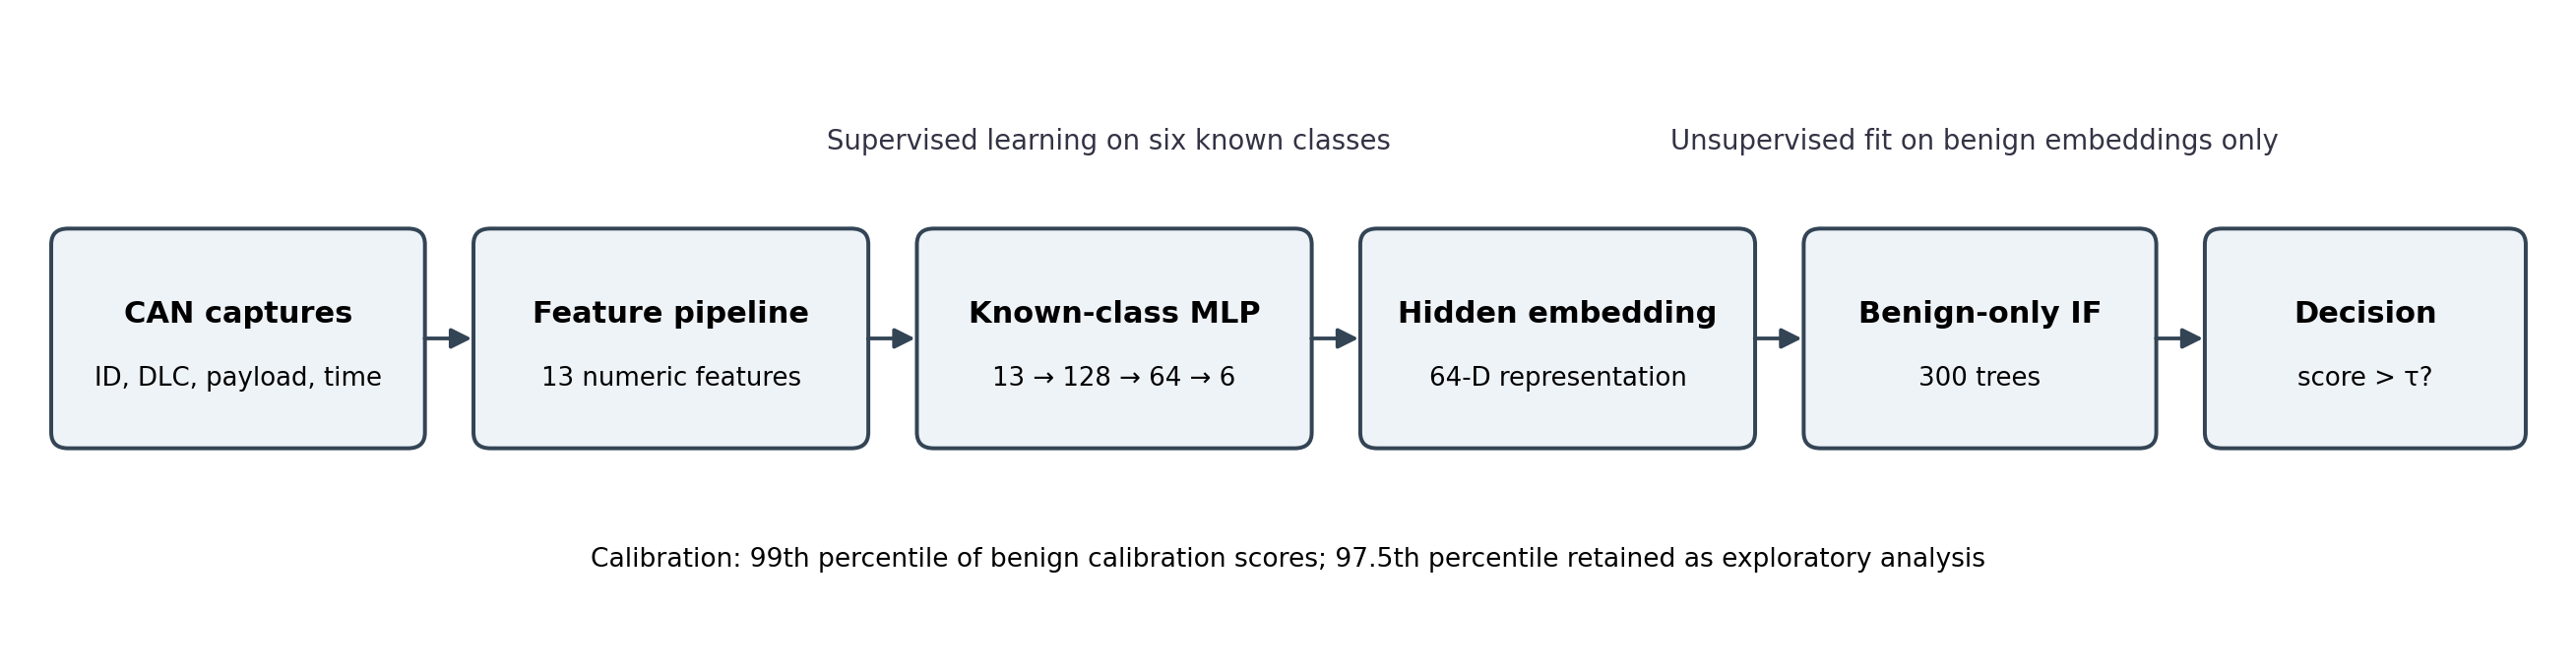
\includegraphics[width=0.98\textwidth]{images/pipeline.png}
\caption{Implemented MLP-representation and benign-only Isolation Forest pipeline. The MLP uses the six known labels; the IF fitting and primary threshold estimation use benign records only.}
\label{fig:pipeline}
\end{figure*}

The data flow contains two different learning objectives. The MLP is supervised: its purpose is to discriminate among the known labels. The IF is unsupervised with respect to attacks: it is fitted only to benign representations and does not use known-attack labels. The two objectives should not be conflated. In particular, the IF is not trained to classify DOUBLE, FUZZING, INTERVAL, SPEED, SYSTEMATIC, or TRIPLE.

\subsection{Multilayer Perceptron}
The MLP receives the 13 standardised features. Its fully connected network has a first hidden layer with 128 units, a ReLU activation, and dropout of 0.2; a second hidden layer with 64 units, another ReLU activation and dropout of 0.2; and a six-unit linear output layer. The architecture can be written as
\begin{align}
 \mathbf{h}_1 &= \mathrm{Dropout}_{0.2}(\mathrm{ReLU}(W_1\mathbf{x}+\mathbf{b}_1)),\\
 \mathbf{h}_2 &= \mathrm{Dropout}_{0.2}(\mathrm{ReLU}(W_2\mathbf{h}_1+\mathbf{b}_2)),\\
 \boldsymbol{\ell} &= W_3\mathbf{h}_2+\mathbf{b}_3,
\end{align}
where $\boldsymbol{\ell}\in\mathbb{R}^{6}$ contains the class logits. During embedding extraction the network is placed in evaluation mode, so dropout is disabled, and the 64-dimensional activation immediately after the second ReLU is captured. In notation, this activation is $\mathbf{z}=f_{\theta}(\mathbf{x})$.

The training script uses cross-entropy loss with square-root inverse-frequency class weights. If $n_c$ is the number of training records for class $c$ and $N$ is the total number of training records, the unnormalised weight is proportional to $\sqrt{N/(6n_c)}$; the weights are normalised to have mean one. This reduces the contribution imbalance caused by class sizes without applying the full inverse-frequency weighting. Optimisation uses Adam with learning rate 0.001, batch size 4096, and 25 epochs. The random seed is set to 42 for the Python numerical library and the PyTorch model. The MLP is run on CPU in the recorded experiment.

The training log reported a final training accuracy of 99.86\%. This figure is a training-set statistic. It does not measure unknown-attack detection performance and must not be presented as a held-out classification accuracy. The downstream anomaly detector is evaluated separately using the unknown-test file.

\subsection{Extraction of the Hidden Representation}
The activation after the second ReLU is a 64-dimensional vector. The dropout layer follows this activation during MLP training, but embedding extraction is performed with the model in evaluation mode. Consequently, the IF receives the deterministic hidden activation from the trained model rather than the output logits. This choice makes the representation a learned feature map from the original 13-dimensional space to a 64-dimensional space.

The representation has no explicit metric-learning loss or contrastive objective. Its geometry is induced by the six-class cross-entropy objective. This is a design choice, not an assumption that the embedding is optimal for unknown-attack detection. The later evaluation is necessary because the MLP was not trained with an explicit objective to separate every unseen attack from benign activity.

\subsection{Isolation Forest Fitting}
The IF is fitted to the hidden representations of the 433,538 benign training records. Its configuration uses 300 estimators, a maximum sample size of 2,048 per tree, automatic contamination handling, random state 42, and parallel execution. The detector is fitted without attack-labelled records. In scikit-learn's decision-function convention, lower values indicate greater abnormality; the project negates the returned decision function so that a higher stored score corresponds to a more anomalous observation. We denote this oriented score by $s(\mathbf{z})$.

The maximum sample size is substantially smaller than the benign training set. This is consistent with the subsampling design of Isolation Forest, but it means that each tree is built from a subset of the training representations. The ensemble combines the resulting isolation behaviour across trees. The study does not tune the tree count or sample size through a nested validation procedure; the parameters are fixed at the values above.

\subsection{Calibration Rule and Operating Point}
Let $\mathcal{S}_{\mathrm{cal}}^{B}$ be the anomaly scores obtained from benign calibration records. The primary threshold is the empirical 99th percentile:
\begin{equation}
  \tau_{99}=Q_{0.99}(\mathcal{S}_{\mathrm{cal}}^{B})=0.1633390.
  \label{eq:q99}
\end{equation}
A record is flagged when $s(\mathbf{z})>\tau_{99}$. The percentile is selected from a benign reference set, rather than from the distribution of unknown-test attack scores. The intended interpretation is an initial operating point that tolerates a small upper tail of benign calibration scores. The 99th percentile does not guarantee a 1\% false-positive rate on a later capture: shifts in vehicle state, collection conditions, or the capture distribution can change the tail behaviour.

A 97.5th-percentile threshold, $\tau_{97.5}=0.0243811$, is also reported. The numerical threshold is calculated from benign calibration scores. However, the decision to examine and emphasise this more permissive quantile followed earlier inspection of unknown-test metrics. Therefore, the associated evaluation is exploratory. It is included to show threshold sensitivity and to preserve the experimental record, not to replace the primary result or to claim an unbiased improvement.

\subsection{Evaluation Measures}
For the binary task, true positives (TP) are attack records flagged by the detector; false positives (FP) are benign records flagged as anomalous; true negatives (TN) are benign records left unflagged; and false negatives (FN) are attack records left unflagged. The metrics are
\begin{align}
 \mathrm{Precision}&=\frac{TP}{TP+FP},\\
 \mathrm{Recall}&=\frac{TP}{TP+FN},\\
 F_1&=2\frac{\mathrm{Precision}\cdot\mathrm{Recall}}{\mathrm{Precision}+\mathrm{Recall}},\\
 \mathrm{FPR}&=\frac{FP}{FP+TN},\\
 \mathrm{Accuracy}&=\frac{TP+TN}{TP+TN+FP+FN}.
\end{align}
ROC-AUC and average precision (reported as PR-AUC in the project outputs) are calculated from continuous scores rather than binary predictions. This distinction matters because threshold changes alter precision, recall, F1, and FPR but do not alter the ranking of a fixed set of continuous scores. In an imbalanced evaluation, a large true-negative count can keep accuracy high even when many attacks are missed. Precision--recall measures are therefore reported with ROC-AUC and the confusion matrix \cite{davis2006prroc}.

\section{Experimental Setup and Baselines}
\subsection{Implementation Environment}
The implementation is written in Python and uses PyTorch for the MLP, scikit-learn for feature standardisation and Isolation Forest, and pandas/NumPy for data handling. The recorded neural-network run used CPU execution, batch size 4096, 25 epochs, and learning rate 0.001. The IF used 300 trees and 2,048 samples per tree. A fixed random seed of 42 was specified in the principal scripts. The package list is supplied separately in \texttt{requirements.txt} in the project repository.

The raw dataset is not redistributed with the research project. Reproduction requires obtaining the dataset from its maintainers, arranging the relevant capture files in the expected directory, and running the preprocessing script to regenerate the processed CSV files. Trained model checkpoints and local intermediate files are not part of the source package. Accordingly, the manuscript reports the outputs obtained in the project environment; it does not claim that a clean machine can reproduce every numeric result without first obtaining the data and rerunning the pipeline.

\subsection{Original-Feature Isolation Forest}
The first comparison model is an IF fitted directly to the original 13-dimensional feature vectors. It uses the benign training rows for fitting and benign calibration scores for the 99th-percentile threshold. The IF parameters are 300 estimators, maximum sample size 2,048, automatic contamination, and random state 42. This comparison helps answer whether the learned representation changes anomaly-score ranking relative to the raw numeric inputs. It is not a comparison against the full set of state-of-the-art CAN IDS methods.

\subsection{Energy-Based OOD Experiments}
The project also executed a six-class MLP energy-score experiment. For logits $\boldsymbol{\ell}(\mathbf{x})$, the score follows
\begin{equation}
 E(\mathbf{x})=-T\log\sum_{k=1}^{6}\exp(\ell_k(\mathbf{x})/T),
 \label{eq:energy}
\end{equation}
with temperature $T=1$. The project evaluated a benign-calibration threshold policy and a maximum-training-malicious-energy adaptation inspired by the unknown-detection discussion in FedGAN-ID. Neither of these executed energy experiments flagged any unknown attack records at the reported operating points. This result is useful as a negative comparison, but it does not establish that energy-based OOD methods generally fail. It only describes these particular model outputs and threshold policies on this evaluation file.

\subsection{Comparison Protocol}
All methods in Table~\ref{tab:comparison} were evaluated on the same processed unknown-test file. The primary comparison uses the 99th percentile for the raw-feature IF and embedding IF. The 97.5th-percentile embedding result is separated with an asterisk because it is exploratory. The energy methods are included as executed project experiments. Direct comparison to FedGAN-ID is intentionally excluded: FedGAN-ID uses a different private vehicle dataset, different attack taxonomy, graph construction, GAN, federated aggregation and privacy mechanisms. Without a common benchmark and protocol, a numeric ranking between the two systems would be misleading.

\section{Results}
\subsection{Primary Result at the 99th Percentile}
At $\tau_{99}=0.1633390$, the embedding detector produces 3,956 true positives, 8,937 false positives, 852,507 true negatives, and 16,869 false negatives. These counts give 30.68\% precision, 19.00\% recall, and an F1-score of 23.47\%. The false-positive rate is 1.04\%, while accuracy is 97.08\%. The accuracy value is not sufficient to describe the detector: the number of benign records is much larger than the number of attacks, and the detector misses more than four-fifths of the attack records at this operating point.

\begin{table}[!t]
\caption{Primary Binary Detection Result at the 99th-Percentile Threshold}
\label{tab:primary}
\centering\footnotesize
\begin{tabular}{lr}
\toprule
Measure & Value\\
\midrule
Threshold & 0.1633390\\
Accuracy & 97.08\%\\
Precision & 30.68\%\\
Recall & 19.00\%\\
F1-score & 23.47\%\\
False-positive rate & 1.04\%\\
ROC-AUC & 0.9423\\
PR-AUC / average precision & 0.4299\\
TP / FP & 3,956 / 8,937\\
TN / FN & 852,507 / 16,869\\
\bottomrule
\end{tabular}
\end{table}

The relatively high ROC-AUC and lower threshold-specific recall are not contradictory. ROC-AUC measures the ranking of positive and negative records across possible cut-offs. The 99th-percentile rule chooses one cut-off from benign calibration data. If attack scores are often higher than benign scores but still fall below that cut-off, the model can obtain a strong ranking measure while returning a low recall at the selected operating point. The converse operational issue is also visible: moving the cut-off lower identifies more attack records but increases the number of benign records raised as alerts.

\subsection{Per-Family Detection at the Primary Threshold}
The aggregate recall of 19.00\% conceals large differences among attack families. FUZZING contributes 3,900 detected records out of 5,975, giving 65.27\% recall. SYSTEMATIC contributes 56 detections out of 1,043, or 5.37\%. No records from DOUBLE, INTERVAL, SPEED, or TRIPLE exceed the primary threshold. Table~\ref{tab:familyprimary} gives the counts and recalls.

\begin{table}[!t]
\caption{Unknown Attack-Family Results at the Primary Threshold}
\label{tab:familyprimary}
\centering\footnotesize
\begin{tabular}{lrr}
\toprule
Family & Detected / total & Recall\\
\midrule
DOUBLE & 0 / 1,292 & 0.00\%\\
FUZZING & 3,900 / 5,975 & 65.27\%\\
INTERVAL & 0 / 4,418 & 0.00\%\\
SPEED & 0 / 5,321 & 0.00\%\\
SYSTEMATIC & 56 / 1,043 & 5.37\%\\
TRIPLE & 0 / 2,776 & 0.00\%\\
\bottomrule
\end{tabular}
\end{table}

The zero-recall outcomes should not be interpreted as proof that the corresponding families are indistinguishable from benign traffic under every feature representation. They indicate that, with this feature set, this trained network, this IF configuration, and the primary threshold, none of the evaluated records in those four families crossed the decision boundary. The result identifies a concrete weakness in this configuration and motivates family-specific analysis rather than a broad claim that unseen CAN attacks are detected reliably.

\subsection{Threshold Sensitivity: Exploratory 97.5th Percentile}
The exploratory threshold is $\tau_{97.5}=0.0243811$. At this value the detector flags 13,022 attacks and 18,905 benign records, yielding 62.53\% recall, 40.79\% precision, 49.37\% F1, and a 2.19\% false-positive rate. Recall increases by 43.53 percentage points relative to the primary operating point; FPR increases by approximately 1.15 percentage points. The number of detected attack records rises by 9,066, while the number of false alerts rises by 9,968.

This is a meaningful change in the alert burden, not a free increase in detector quality. The 97.5th-percentile result may be attractive where missed attacks are considered more costly than additional alerts, but that operational preference would need to be defined before examining the test labels. In this study, the unknown-test file was inspected during earlier threshold exploration. As a result, the selected 97.5th-percentile point is reported transparently as exploratory and should not be used as the headline validated performance figure.

At this exploratory operating point, family-wise recall is 9.06\% for DOUBLE, 80.52\% for FUZZING, 96.42\% for INTERVAL, 60.27\% for SPEED, 34.32\% for SYSTEMATIC, and 9.69\% for TRIPLE. The gain is therefore not evenly distributed. INTERVAL and SPEED change from zero recall at the primary threshold to high or moderate recall at the exploratory threshold, while DOUBLE and TRIPLE remain difficult. Fig.~\ref{fig:families} presents both sets of family-wise results.

\begin{figure}[!t]
\centering
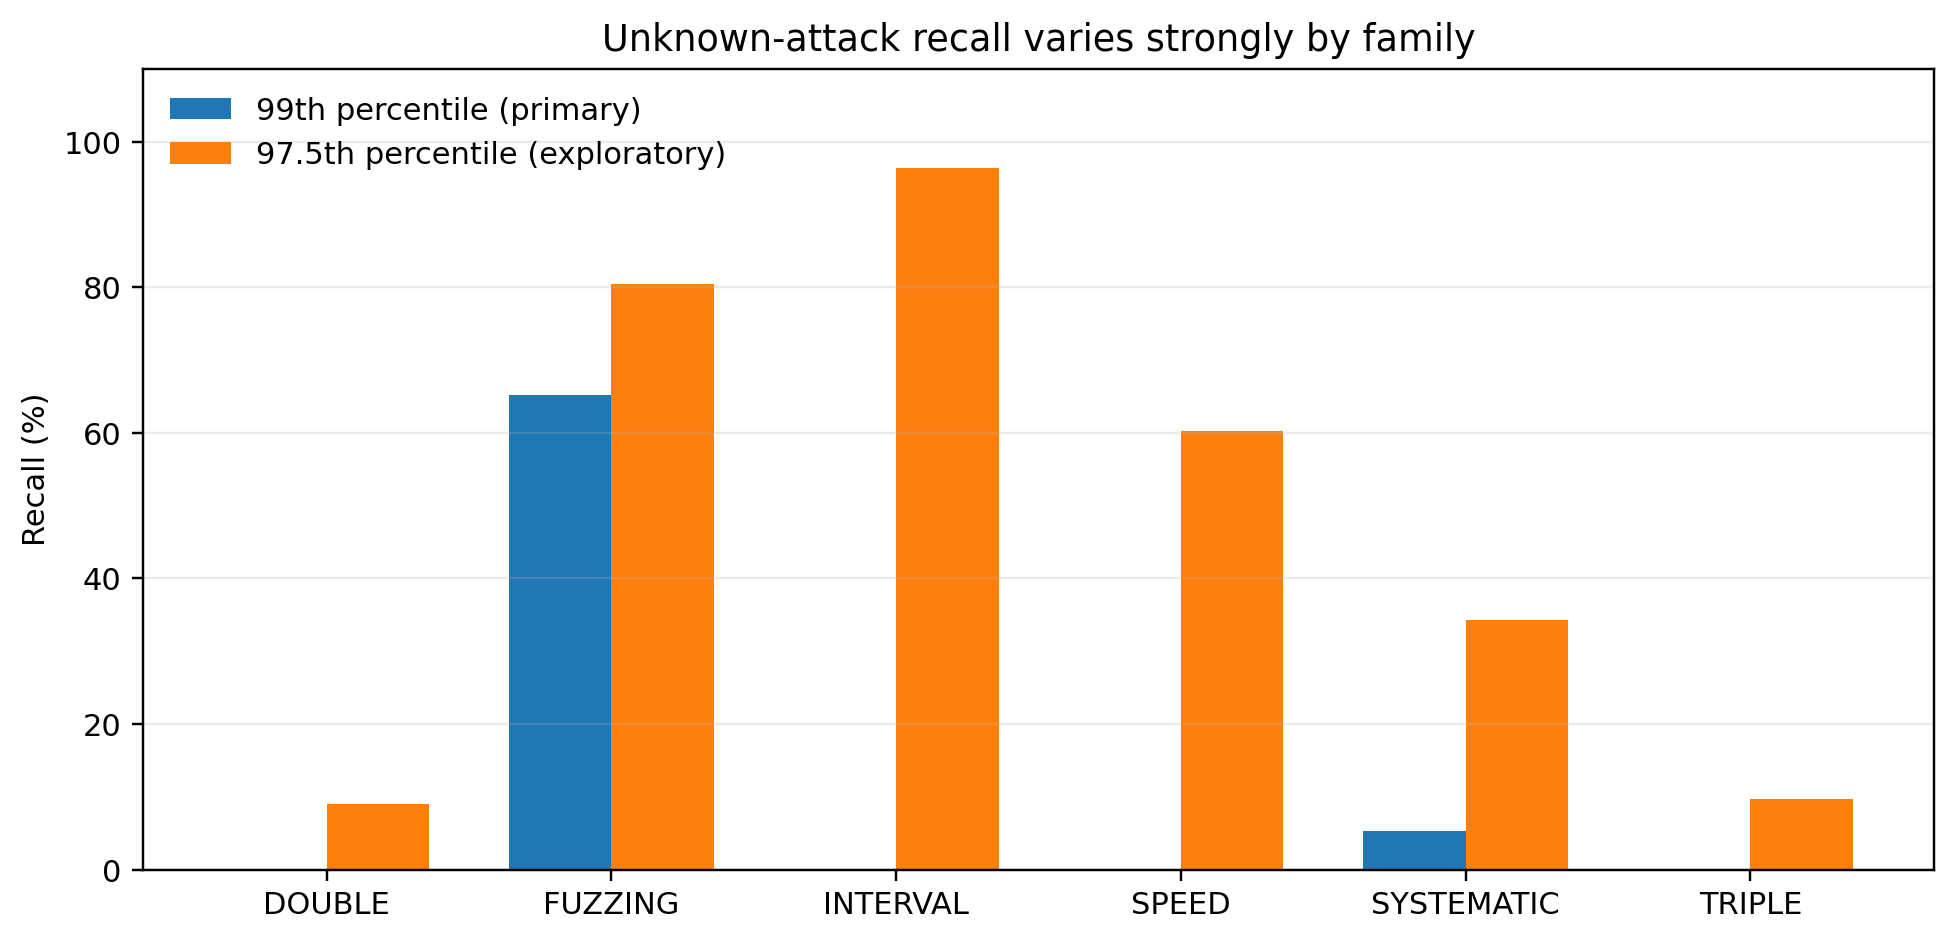
\includegraphics[width=\columnwidth]{images/family_recall.png}
\caption{Recall by unknown attack family at the primary 99th-percentile and exploratory 97.5th-percentile thresholds.}
\label{fig:families}
\end{figure}

\begin{table}[!t]
\caption{Primary and Exploratory Operating Points}
\label{tab:thresholds}
\centering\footnotesize
\begin{tabular}{lrr}
\toprule
Metric & 99th (primary) & 97.5th (exploratory)\\
\midrule
Threshold & 0.1633390 & 0.0243811\\
Accuracy & 97.08\% & 96.97\%\\
Precision & 30.68\% & 40.79\%\\
Recall & 19.00\% & 62.53\%\\
F1-score & 23.47\% & 49.37\%\\
FPR & 1.04\% & 2.19\%\\
ROC-AUC & 0.9423 & 0.9423\\
PR-AUC & 0.4299 & 0.4299\\
TP & 3,956 & 13,022\\
FP & 8,937 & 18,905\\
FN & 16,869 & 7,803\\
TN & 852,507 & 842,539\\
\bottomrule
\end{tabular}
\end{table}

The ROC-AUC and PR-AUC values remain the same between the two threshold rows because both are computed from the same continuous score vector on the same evaluation records. Threshold choice changes the binary predictions, not the score ranking. Reporting the same AUC values beside different F1 values is therefore expected; it is not a separate improvement in ranking.

\begin{figure}[!t]
\centering
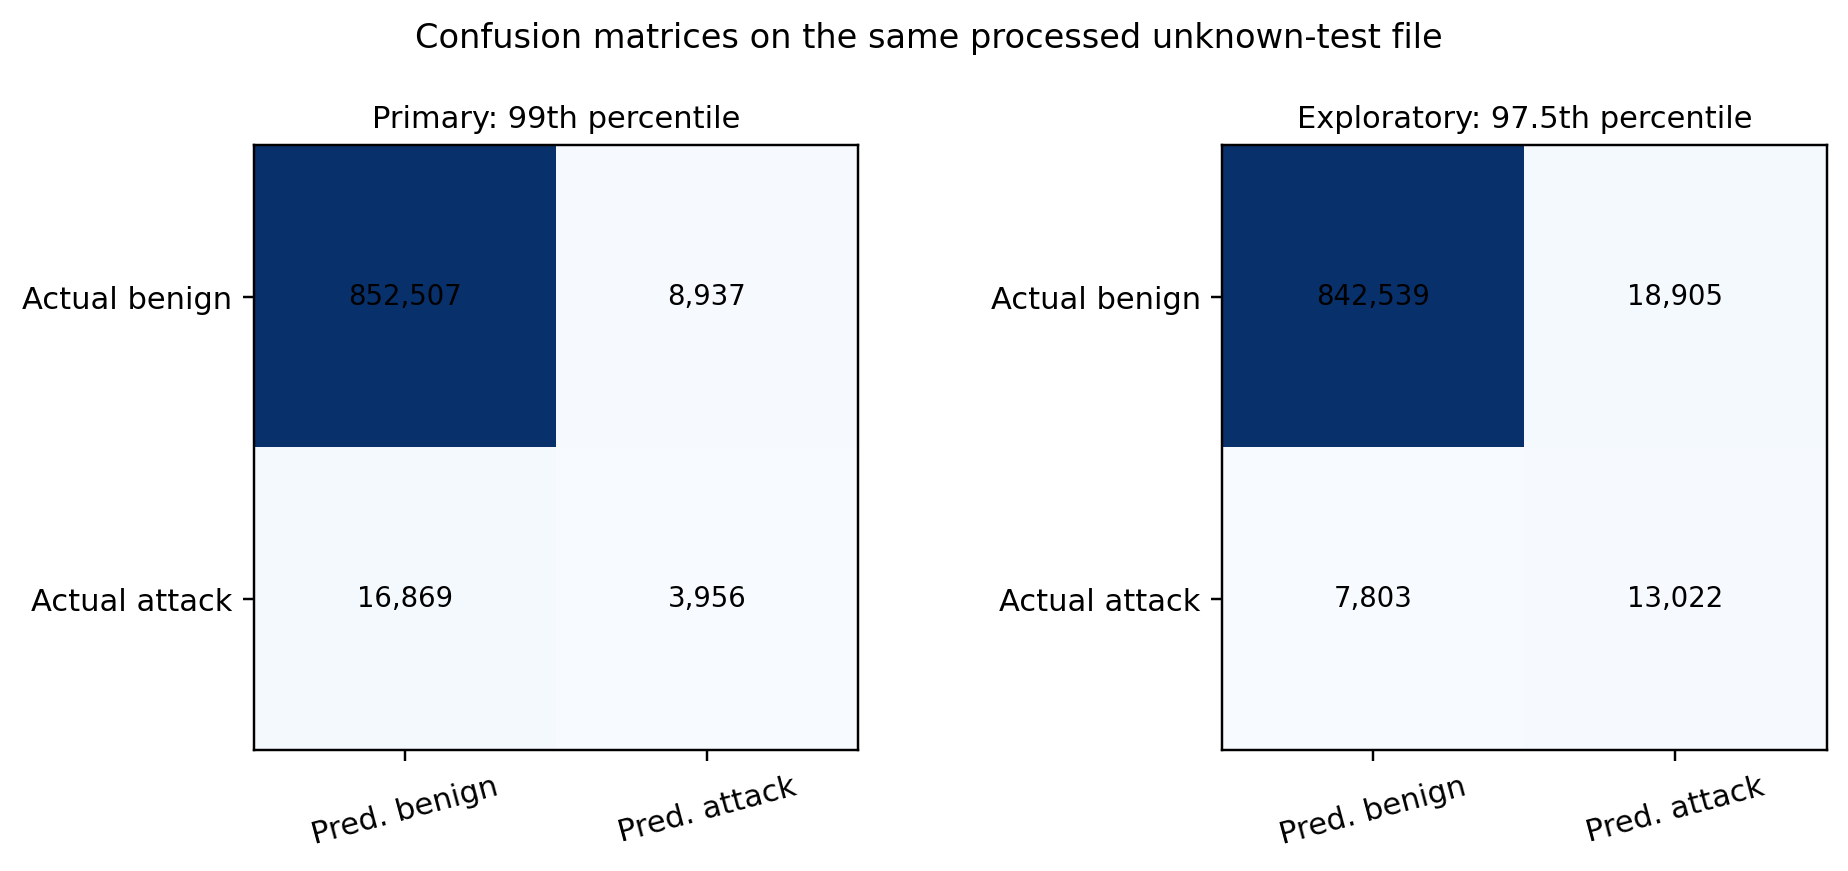
\includegraphics[width=\columnwidth]{images/confusion_matrices.png}
\caption{Confusion matrices for the primary and exploratory operating points. The exploratory panel is included to illustrate threshold sensitivity and is not an independent validation result.}
\label{fig:confusions}
\end{figure}

\subsection{Comparison with the Original-Feature Baseline}
The IF trained on the original 13 features obtains F1 28.94\%, recall 24.47\%, and FPR 1.08\% at its 99th-percentile threshold. The embedding-based IF obtains F1 23.47\%, recall 19.00\%, and FPR 1.04\%. Thus, by the selected threshold-specific metrics, the original-feature IF performs better on F1 and recall, while the embedding detector has a slightly lower FPR.

The ranking measures show a different pattern. The original-feature IF has ROC-AUC 0.6303 and PR-AUC 0.2006, whereas the embedding IF has ROC-AUC 0.9423 and PR-AUC 0.4299. The embedding provides a much stronger ordering of the evaluated benign and attack records according to these area measures. This does not make the embedding detector unambiguously superior. It means its score distribution separates many positive and negative examples in ranking terms, but the selected 99th-percentile cut-off is conservative for this test distribution. A detector selection decision should take account of both ranking quality and the alert rate at the intended operating point.

\begin{table*}[!t]
\caption{Executed Method Comparisons on the Same Unknown-Test File}
\label{tab:comparison}
\centering\footnotesize
\begin{tabular}{lrrrr}
\toprule
Method & F1 & Recall & FPR & ROC-AUC\\
\midrule
Raw-feature IF, 99th & 28.94\% & 24.47\% & 1.08\% & 0.6303\\
Embedding IF, 99th & 23.47\% & 19.00\% & 1.04\% & 0.9423\\
Embedding IF, 97.5th$^*$ & 49.37\% & 62.53\% & 2.19\% & 0.9423\\
Energy OOD & 0.00\% & 0.00\% & 0.001\% & 0.2325\\
Max-training-energy & 0.00\% & 0.00\% & 0.0017\% & 0.2325\\
\bottomrule
\multicolumn{5}{p{0.92\textwidth}}{\scriptsize $^*$Exploratory threshold: the evaluation file had been inspected during earlier threshold analysis. The energy rows describe only the two executed project configurations.}
\end{tabular}
\end{table*}

The energy-based experiments did not detect unknown records at the chosen operating points. Their near-zero FPR is not a useful result by itself because it is accompanied by zero recall. In practical intrusion detection, a detector that never raises an attack alert is not effective merely because it rarely alarms on benign traffic. This negative result is included because it influenced the model-selection process; it should not be generalised to all energy-based OOD methods.

\begin{figure}[!t]
\centering
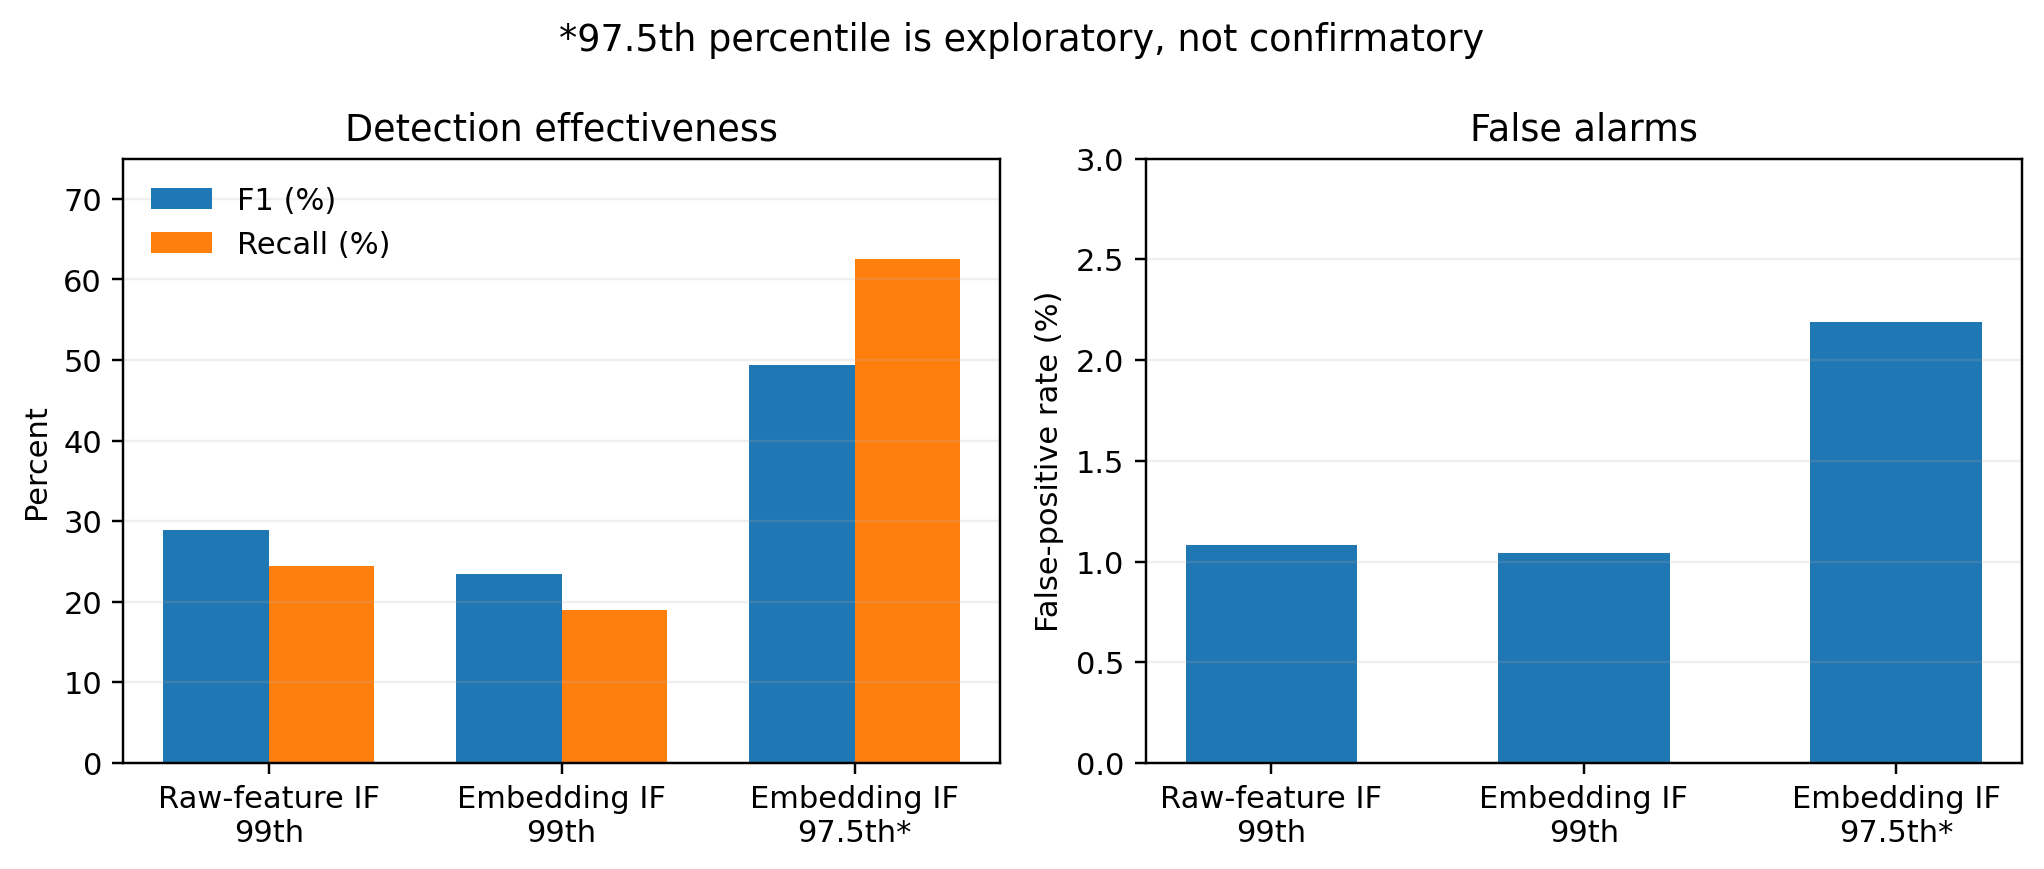
\includegraphics[width=\columnwidth]{images/method_comparison.png}
\caption{Threshold-specific F1, recall, and FPR for the two Isolation Forest configurations. The 97.5th-percentile point is exploratory.}
\label{fig:methodcomparison}
\end{figure}

\subsection{Anomaly-Score Distribution by Family}
The median anomaly score differs across the evaluated labels. The benign median is $-0.131440$. The medians for DOUBLE and TRIPLE are $-0.108853$ and $0.006674$, respectively, while FUZZING has a much higher median of $0.297320$. INTERVAL and SPEED have medians of $0.044970$ and $0.033780$, and SYSTEMATIC has a median of $-0.029677$. These summaries are consistent with the observed recall pattern: FUZZING scores tend to lie further into the anomalous tail, whereas the score distributions for DOUBLE and TRIPLE overlap more strongly with the benign region.

\begin{figure}[!t]
\centering
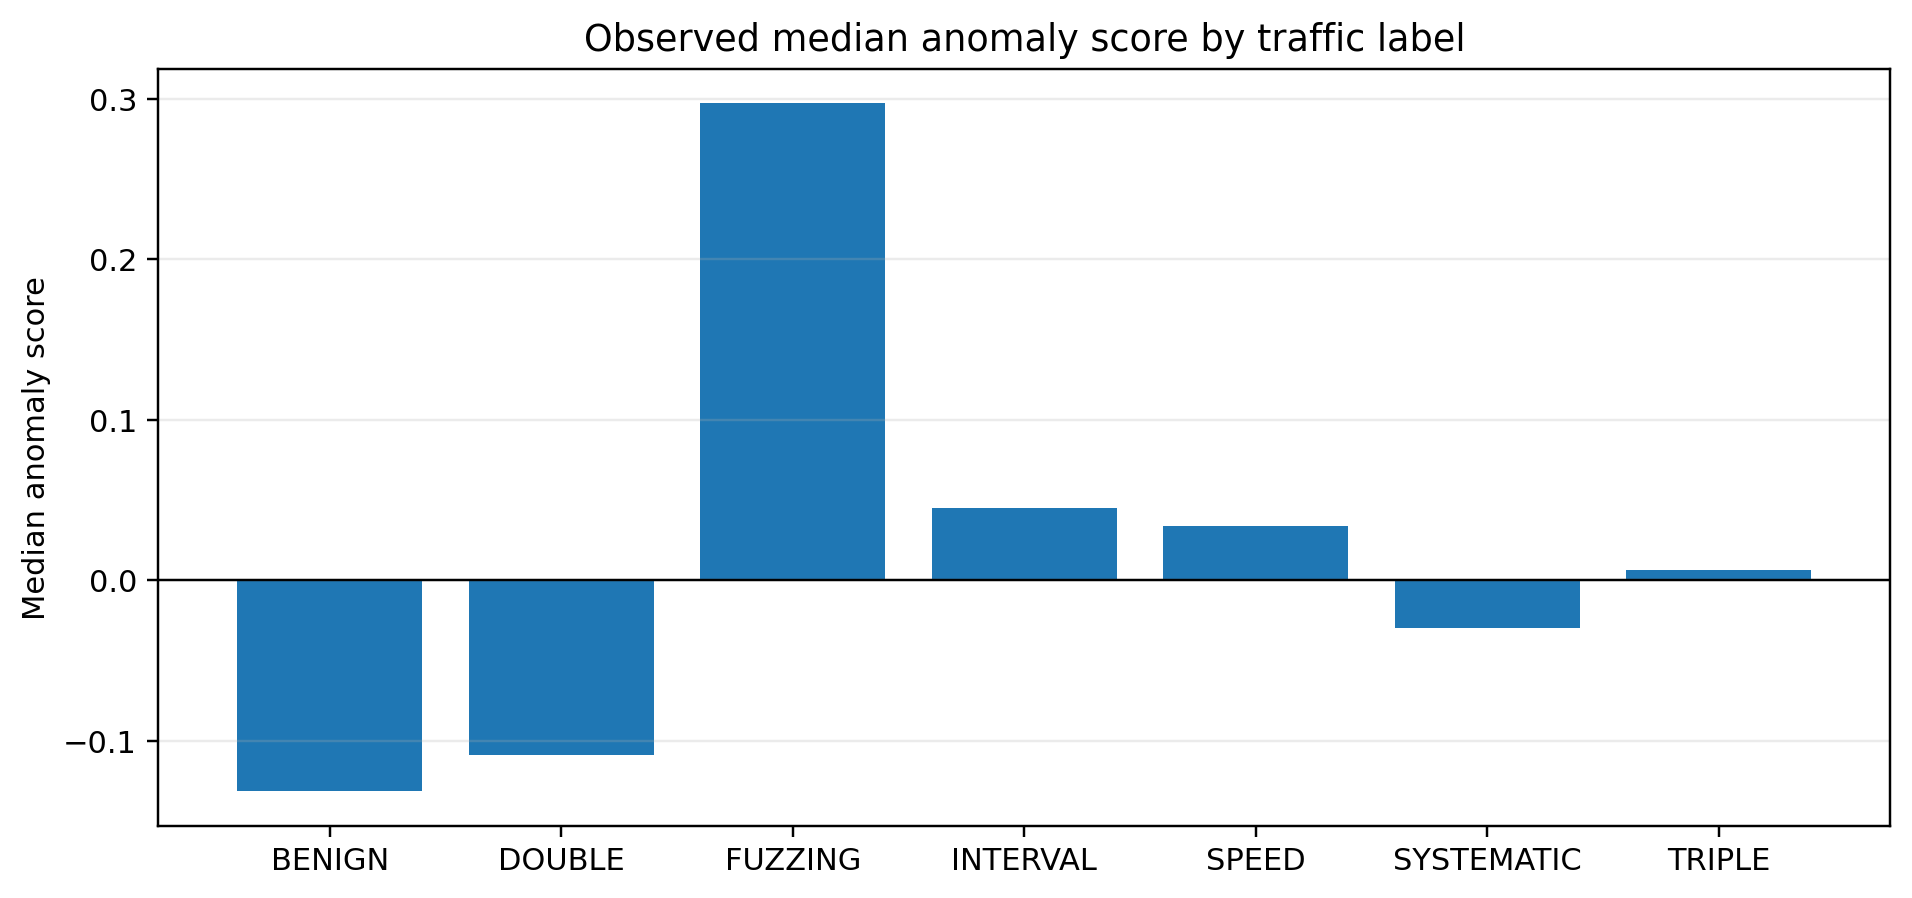
\includegraphics[width=\columnwidth]{images/score_medians.png}
\caption{Median anomaly score by ground-truth group. Higher scores are more anomalous under the stored score convention.}
\label{fig:scoremedians}
\end{figure}

A median is only one point in a distribution. It does not describe the tails, spread, or proportion of records above a selected threshold. Therefore, the median plot is used as a descriptive diagnostic, not as a substitute for the family-wise confusion counts. In particular, a family may have a median below the threshold but still contain a high-scoring subset, and a median above the threshold does not imply that every record is flagged.

\subsection{Timing and Payload Diagnostics}
The processed data also provide timing and payload summaries that help interpret the family-specific outcomes. The benign median inter-arrival time is 0.0138 ms, compared with 0.8030 ms for DOUBLE and 0.7639 ms for TRIPLE. Median payload length is 8 bytes for benign records, 7 for DOUBLE, and 5 for TRIPLE. FUZZING has a median inter-arrival time of 0.8988 ms and a very large median same-identifier inter-arrival time in the processed summary. INTERVAL shows a median inter-arrival time of 0.3589 ms and a same-identifier inter-arrival time of 0.3641 ms. SPEED records show median inter-arrival and same-identifier inter-arrival times of 0.8707 ms and 2.9240 ms, respectively.

These are marginal summaries. They do not demonstrate that a specific timing feature caused a detection or miss. The MLP may combine all input dimensions nonlinearly, and the IF acts on the 64-dimensional representation rather than on an individual feature. A controlled ablation study would be needed to attribute the difference in family recall to timing, payload, or identifier information. No such ablation is claimed in this manuscript.

\section{Discussion}
\subsection{A High AUC Does Not Select an Operating Point}
One of the most important outcomes is the gap between ranking and thresholded performance. The embedding-based detector has a ROC-AUC of 0.9423 and a PR-AUC of 0.4299, but it achieves only 19.00\% recall at the primary 99th-percentile threshold. The score ranking contains useful information, yet the chosen threshold leaves many attack records below the decision boundary. This is not an unusual distinction in imbalanced detection: AUC summarises behaviour across thresholds, whereas a deployed IDS must make a decision at one operating point. The selected operating point should reflect an acceptable balance between missed attacks and false alerts, and should be determined without repeatedly consulting the final evaluation labels \cite{davis2006prroc}.

A lower threshold can increase detection by accepting a larger benign tail. In this experiment the move from the 99th to the 97.5th percentile increases the recall from 19.00\% to 62.53\%, but also increases FPR from 1.04\% to 2.19\%. For a large volume of legitimate messages, even a small percentage-point increase in FPR can create a substantial alert count. Conversely, a conservative operating point can miss attacks that only weakly depart from the benign representation distribution. A real deployment would need to choose the operating point from a policy-defined validation set, perhaps using an alert budget or a cost model, and then freeze it before evaluation on a later capture.

\subsection{Why Does Detection Vary by Family?}
The gap between FUZZING and the other families indicates that one binary threshold does not affect all unknown attacks in the same way. FUZZING has a high median anomaly score and the strongest recall at both thresholds. INTERVAL and SPEED also respond to a more permissive threshold, suggesting that many of their records lie between the two cut-offs. DOUBLE and TRIPLE remain difficult even at the exploratory operating point. Their median scores are comparatively close to the benign median, which is consistent with overlap in the representation space.

A plausible explanation is that some attack families change timing or payload patterns in ways that are visible to the learned representation, while other families produce records whose 13 input values remain close to common benign traffic. This is a hypothesis, not a demonstrated causal mechanism. The present experiments do not include feature ablations, sequence-level models, or class-conditional embedding visualisations that would establish why a particular family is missed. For now, the family-wise count table is the strongest evidence: it records which groups cross the threshold without assigning a cause that the experiment did not isolate.

\subsection{Representation Learning Can Help Ranking Without Improving F1}
The raw-feature IF baseline offers an important counterpoint to the representation-based result. At the 99th percentile, the raw-feature detector has better F1 and recall even though its ROC-AUC and PR-AUC are lower. One interpretation is that the MLP representation improves the ordering of many attack records relative to benign records, but the calibration percentile and scale of the score distribution result in a cut-off that is poorly positioned for the particular test capture. Another possibility is that a few groups of attack records become much easier to rank, while other groups remain close to benign traffic. The family-wise results are consistent with the latter possibility, but a decomposition of the full score distribution would be needed to quantify each group's contribution to the AUC.

This distinction cautions against describing a learned embedding as an improvement solely because it produces a larger AUC. The outcome depends on what is being optimised. If the operational requirement is to maintain a low FPR at a specified budget, the threshold-specific metrics matter. If the requirement is to support later calibration or analyst triage, ranking quality may also matter. A useful evaluation should report both rather than selecting whichever metric makes the method look strongest.

\subsection{What the Failed Energy Experiments Tell Us}
The energy-based experiments yielded no detections at their reported thresholds. Their scores therefore failed to produce a useful operating point in this configuration. The result highlights the sensitivity of OOD detection to the classifier's learned logits and the choice of threshold. An input from an unknown attack family can still produce logits that are confidently assigned to one of the known classes; the energy score is then not guaranteed to be large. This is a possible explanation for the observed failure, but the project did not conduct an experiment that directly verifies the confidence mechanism for each unknown family.

FedGAN-ID uses an energy-based unknown-attack mechanism within a larger system that includes a GAN-based detector, a graph representation, and federated learning \cite{chen2025fedgan}. The local energy experiments here are not an implementation of that complete approach. They also do not establish that the full FedGAN-ID design would fail on this dataset. A method-level comparison requires implementing the same architecture and evaluating it under a shared protocol, or at least carefully matching datasets and thresholds. Neither condition is met.

\subsection{Calibration Under Distribution Shift}
The 99th-percentile calibration rule is simple and reproducible: it fixes the threshold from the upper tail of benign calibration scores. Its weakness is that the calibration and test score distributions may differ. A new driving session, a different vehicle, changed bus load, maintenance activity, or a modified capture setup may shift the benign score distribution. A threshold that corresponds to one percent of benign calibration scores can therefore produce a different false-positive rate elsewhere. This study observes a 1.04\% FPR on the processed test file, which is close to but not guaranteed by the 99th-percentile calibration rule.

An operational calibration procedure should test stability over multiple benign sessions and vehicles. It should also include a method for handling drift. Updating a threshold automatically is not straightforward: if the data used for recalibration contain undetected attacks, the benign reference region may be contaminated. Future work should investigate drift detection and controlled recalibration with trusted benign intervals rather than treating a single calibration percentile as a universal constant.

\subsection{Implications for a Vehicle IDS}
The implemented pipeline can be understood as a research prototype for record-level anomaly scoring. It has not been evaluated on an automotive electronic control unit, a production gateway, or a hardware-in-the-loop setup. The reported training time and offline processing do not establish real-time inference feasibility. A deployment study would need to measure per-frame latency, throughput under bus load, memory consumption, model update cost, and the effect of logging and preprocessing on an embedded processor. It would also need to test whether timing features can be calculated with consistent semantics in the target gateway.

A further distinction concerns alerts. The current output is binary and does not identify the originating ECU or explain which byte or timing feature caused the score. For use by a vehicle-security engineer, an alert would ideally include contextual evidence: identifier, capture time, local score, threshold, surrounding frames, and a confidence or severity interpretation. That extension must be designed carefully so that explanation does not create false confidence or disclose sensitive vehicle information.

\section{Validity Considerations and Limitations}
Several limitations determine how far the results can be generalised.

\subsection{Evaluation-Set Reuse}
The unknown-test file was examined during earlier exploratory threshold analysis. Even though the threshold value is calculated from benign calibration scores, the decision to emphasise the 97.5th percentile followed inspection of test performance. This creates a model-selection concern: the exploratory result is no longer an untouched estimate of generalisation. The 99th-percentile operating point is retained as the primary result because it was the initially selected operating point. A new capture that has not been consulted during development is required for an independent estimate.

\subsection{Class Prevalence and Sampling}
Benign traffic was subsampled while attack records were retained. The unknown-test file has an attack prevalence of approximately 2.36\%. Precision and accuracy depend on class prevalence, so they should not be transferred directly to a deployment environment with a different benign-to-attack ratio. Recall and FPR are also subject to dataset and capture shift. The sampling policy must be disclosed when using the reported precision and accuracy in a comparison.

\subsection{Limited Dataset and Capture Scope}
The experiments use one configured known-class training/calibration workflow and one designated unknown-attack test file. They do not establish performance over all vehicles, software versions, road conditions, and bus configurations. The can-train-and-test paper was designed to support broader comparisons across attack types and vehicles, but this project has not run all of its subsets \cite{lampe2024dataset}. Consequently, no universal cross-vehicle claim is made.

\subsection{Single Configuration and Randomness}
The reported model uses a fixed seed and one configured training run. There are no multi-seed means, standard deviations, confidence intervals, or statistical significance tests. The IF itself uses random partitioning. Although fixed random states make the recorded run more repeatable, they do not show how stable the performance is across different seeds. A stronger study would repeat the full pipeline using several seeds and report variation in both aggregate and family-wise metrics.

\subsection{Representation and Feature Limitations}
The MLP is trained for six-class classification, not for open-set representation learning. The hidden space may suppress variations that do not help separate the known classes. The 13-dimensional input contains only a small set of per-frame and local timing attributes. It does not include a learned graph of message transitions, a longer sequence window, physical-layer information, or explicit transmitter identity. Numeric CAN identifier encoding may also impose distances that do not reflect semantic relations among message IDs.

\subsection{No Complete FedGAN-ID Reproduction}
The work does not implement the GAN, federated aggregation, differential privacy, message-graph construction, MTF, READ, or the second-level classifier described in FedGAN-ID. It also does not evaluate privacy leakage, communication overhead, client heterogeneity, or attack detection latency on a real vehicle. The use of FedGAN-ID as motivation must not be interpreted as proof that the present project reproduces the article's architecture or validates its reported results \cite{chen2025fedgan}.

\subsection{No Independent Similarity or AI-Authorship Certification}
The manuscript reports experimental measurements from the project and cites the sources used to describe prior methods and the dataset. The authors should still review every paragraph, check that each statement is supported by the cited source or experiment, and follow their institution's rules for disclosing writing tools. Text similarity and AI-writing indicators are different forms of assessment and neither substitutes for a manual check of quotation, attribution, authorship, and research records. No numerical claim about plagiarism or AI authorship can be made from the model's experimental outputs.

\section{Reproducibility and Reporting Checklist}
To make a future rerun easier to audit, the following items should accompany the paper: (i) the exact repository commit used for the submitted manuscript; (ii) the dataset version and capture filenames; (iii) the preprocessing script and its sampling settings; (iv) the Python and library versions; (v) the MLP checkpoint and scaler or an instruction to regenerate them; (vi) the seed and training parameters; (vii) the exact calibration file and benign-row filtering rule; (viii) the IF configuration and threshold percentile; and (ix) the scripts that generate every reported table and figure. The raw dataset should be obtained from its maintainers rather than redistributed without checking its licence.

A reproducibility package should distinguish source code from generated outputs. The scripts and configuration are necessary to reproduce the analysis, while the CSV result summaries and figures are convenient evidence of the particular run. A clean installation test should start from the repository root, recreate the environment, run preprocessing, train the model, extract embeddings, fit the detector, and execute evaluation. A syntax check alone is not a runtime reproduction. The current manuscript therefore describes the implementation and its recorded outputs without claiming that a third party has independently rerun the complete workflow.

\section{Future Work}
A first priority is to obtain an untouched evaluation capture. The threshold percentile, feature set, and model configuration should be frozen using training and validation data only. The final capture should be opened only after the complete decision rule is fixed. This would provide a cleaner estimate of whether the 99th-percentile operating point transfers to a new session and whether a more permissive threshold is justified by a predeclared alert budget.

A second direction is to evaluate the effect of the input representation. Ablations could remove payload bytes, CAN identifier, or each timing feature group in turn. A temporal model could process a sequence of consecutive records rather than independent row vectors. A graph-based model could represent message transitions or co-occurrence patterns. These experiments would help test the hypothesis that DOUBLE and TRIPLE are difficult because their local feature distributions overlap with benign traffic. Such an explanation should only be accepted if the controlled experiments support it.

Third, the threshold should be evaluated as an operational parameter. Instead of selecting a percentile after observing test results, the study could choose a target benign alert rate on a validation set, freeze the threshold, and report its performance across separate captures. Calibration stability should be measured by vehicle, session, and operating condition. The model should also be assessed using precision--recall curves, family-wise metrics, and confidence intervals across repeated training runs.

Fourth, the energy-based baseline should be investigated with a controlled study of logit distributions and threshold policies. The present zero-recall outcome suggests that the current energy score is not separating the unknown attack examples at the tested threshold. It does not reveal whether the issue is the MLP, the score definition, the temperature, the calibration population, or the attack distribution. These factors should be varied one at a time on validation data before any claim is made.

Finally, federated and privacy-preserving extensions could be explored if multiple vehicle datasets become available. Such an extension would require a true multi-client setup, explicit local training and aggregation, a documented privacy mechanism and budget, and analysis of the effect of privacy noise on anomaly detection. Those are substantial additional experiments; they are not minor modifications to the current IF pipeline.

\section{Conclusion}
This paper has examined a neural-representation and benign-only Isolation Forest pipeline for identifying attack records excluded from the MLP's known-class training labels. The primary threshold is the 99th percentile of benign calibration anomaly scores. On the evaluated unknown-attack file, it yields 30.68\% precision, 19.00\% recall, 23.47\% F1, and a 1.04\% false-positive rate. Continuous scores achieve ROC-AUC 0.9423 and PR-AUC 0.4299. Family-wise analysis shows that the primary threshold detects FUZZING more often than the other unknown families and misses all evaluated DOUBLE, INTERVAL, SPEED, and TRIPLE records.

The original-feature IF baseline has a higher F1-score at its 99th-percentile operating point, while the embedding IF has higher ROC-AUC and PR-AUC. This difference demonstrates why ranking metrics and threshold-specific measures should be read together. The 97.5th-percentile threshold raises recall to 62.53\% and F1 to 49.37\%, but it also increases the false-positive rate to 2.19\% and remains exploratory because the test file was inspected during earlier threshold analysis. It is not presented as an independent performance estimate.

The experiment offers a practical record of what this implementation detects and what it misses. It does not show that the complete FedGAN-ID system has been reproduced, and it does not demonstrate the GAN, federated learning, differential privacy, graph construction, or message-level modules of that paper. The most important next step is a fresh, untouched evaluation capture combined with repeated runs and a threshold policy fixed before test evaluation. Until that work is completed, the reported values should be treated as dataset-specific experimental evidence rather than a deployment guarantee.

\section*{Acknowledgment}
The authors thank Dr. Bhale Pradeepkumar Gajendra for guidance during the research project. The authors are responsible for verifying the correctness of the experiments, interpreting the results, and ensuring that the final manuscript complies with the institution's research and authorship policies.

\balance
\bibliographystyle{IEEEtran}
\bibliography{references}
\end{document}
